\begin{figure}[H]
    \centering
    

\tikzset{every picture/.style={line width=0.75pt}} %set default line width to 0.75pt        

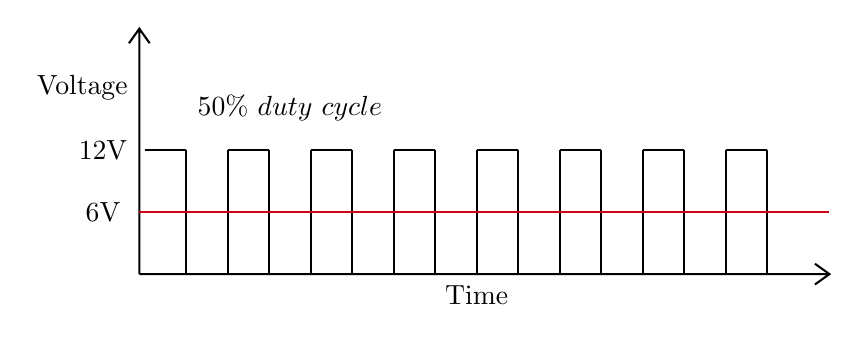
\begin{tikzpicture}[x=0.75pt,y=0.75pt,yscale=-1,xscale=1]
%uncomment if require: \path (0,195.7708282470703); %set diagram left start at 0, and has height of 195.7708282470703

%Shape: Axis 2D [id:dp4590371439594336] 
\draw  (67.5,160) -- (400,160)(67.5,41.77) -- (67.5,160) -- cycle (393,155) -- (400,160) -- (393,165) (62.5,48.77) -- (67.5,41.77) -- (72.5,48.77)  ;
%Straight Lines [id:da2226440769036555] 
\draw    (70,100) -- (90,100) ;


%Straight Lines [id:da027973599787850967] 
\draw    (110,100) -- (130,100) ;


%Straight Lines [id:da43134384380494617] 
\draw    (150,100) -- (170,100) ;


%Straight Lines [id:da4567622353820677] 
\draw    (190,100) -- (210,100) ;


%Straight Lines [id:da06280461715383967] 
\draw    (230,100) -- (250,100) ;


%Straight Lines [id:da7961110488444294] 
\draw    (270,100) -- (290,100) ;


%Straight Lines [id:da2952115332924481] 
\draw    (310,100) -- (330,100) ;


%Straight Lines [id:da347939513568553] 
\draw    (350,100) -- (370,100) ;


%Straight Lines [id:da5371311326985915] 
\draw    (90,100) -- (90,160) ;


%Straight Lines [id:da37558688962973075] 
\draw    (110,100) -- (110,160) ;


%Straight Lines [id:da44168060142753496] 
\draw    (130,100) -- (130,160) ;


%Straight Lines [id:da5162984720027333] 
\draw    (170,100) -- (170,160) ;


%Straight Lines [id:da9328655937237107] 
\draw    (150,100) -- (150,160) ;


%Straight Lines [id:da8698526285458617] 
\draw    (190,100) -- (190,160) ;


%Straight Lines [id:da5579333462058347] 
\draw    (210,100) -- (210,160) ;


%Straight Lines [id:da2831852027876949] 
\draw    (230,100) -- (230,160) ;


%Straight Lines [id:da9724068952844995] 
\draw    (270,100) -- (270,160) ;


%Straight Lines [id:da36611358171538266] 
\draw    (250,100) -- (250,160) ;


%Straight Lines [id:da1948477680776879] 
\draw    (290,100) -- (290,160) ;


%Straight Lines [id:da11576257223436737] 
\draw    (310,100) -- (310,160) ;


%Straight Lines [id:da05602527791808809] 
\draw    (330,100) -- (330,160) ;


%Straight Lines [id:da33311457706338143] 
\draw    (370,100) -- (370,160) ;


%Straight Lines [id:da13026763207224157] 
\draw    (350,100) -- (350,160) ;


%Straight Lines [id:da8029430980655885] 
\draw [color={rgb, 255:red, 208; green, 2; blue, 27 }  ,draw opacity=1 ]   (67.5,130) -- (400,130) ;



% Text Node
\draw (40,70) node  [align=left] {Voltage};
% Text Node
\draw (230,170) node  [align=left] {Time};
% Text Node
\draw (140,80) node   {$50\%\ duty\ cycle$};
% Text Node
\draw (50,100) node  [align=left] {12V};
% Text Node
\draw (50,130) node  [align=left] {6V};


\end{tikzpicture}
    \caption{Illustration of Voltage over time with PWM between 0 and 12V with a duty cycle of 50\%. The read line indicates the average voltage of 6V received by a device}
    \label{fig:PWMUCH}
\end{figure}